\section{繪圖與渲染實作}

\subsection{基本圖形}

每種幾何圖形都能提供 Renderer 所需的頂點。Line 回傳兩端點，Rectangle 回傳四個角，Ellipse 以固定 64 個 segment 取樣，Path 與 Polygon 則使用工具收集的點。Point 是較簡單的特例，直接以 \lstinline|GL_POINTS| 和目前的 point size 繪製。Renderer 因此只需要處理完成後的 geometry，不用知道前面是單擊、拖曳還是多次點擊。

\subsection{Interactive Drawing 與 Draft}

繪圖工具不會在 Mouse Down 時立刻修改 Document，而是先建立一個 draft。接下來的 Motion 只改變 draft 的座標並要求重畫，所以使用者可以立即看到預覽。直到 Mouse Up、DoubleClick 或 Enter 表示操作完成，Canvas 才把新物件交給 Document 與 Command History。圖~\ref{fig:drawing-lifecycle} 是 DragTool 和 PolygonTool 共用的主要流程。

\begin{figure}[tbp]
    \centering
    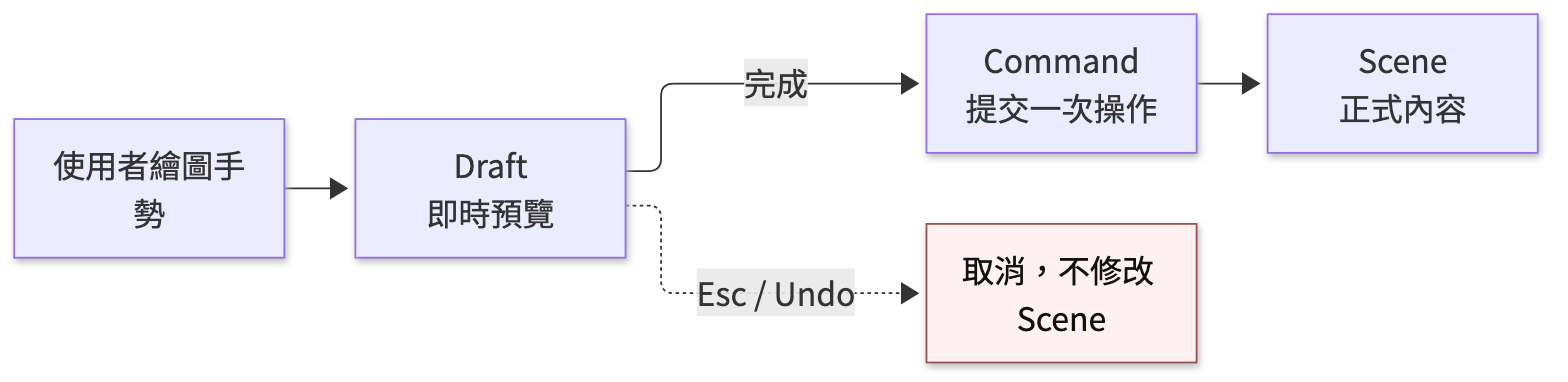
\includegraphics[width=.98\textwidth]{docs/figures/ch04_drawing-lifecycle.png}
    \caption{繪圖工具與草稿的生命週期}
    \label{fig:drawing-lifecycle}
\end{figure}

切換工具時，目前工具會先處理尚未完成的 draft。若使用者在互動過程中按下 Undo，程式先取消 draft，而不是立刻復原 Scene 中上一個物件。這讓「取消這次尚未完成的動作」和「復原前一次已完成的動作」不會混在一起。

\subsection{物件選取與刪除}
\label{sec:selection-delete}

SelectTool 由 Scene 尾端向前搜尋，也就是先檢查最後繪製的物件。一旦命中就停止搜尋，因此圖形重疊時會優先選到視覺上的最上層物件。文字物件以字型計算出的寬高建立矩形，點擊座標落在矩形內即為命中。

圖形物件先轉成頂點序列。對於「封閉且有可見填色」的圖形，程式以 ray-crossing（even--odd）測試點擊位置是否在多邊形內；每當向右的水平射線穿過一條邊就切換一次內外狀態。這使 Rectangle、Polygon，以及由 64 個 segment 近似的 Ellipse，都能從填色區域內部選取。

只有外框或開放路徑時，則計算點擊點 $P$ 到每條線段 $\overline{AB}$ 的最短距離。令 $\vec{v}=B-A$，投影參數與距離為

\[
    t=\operatorname{clamp}\!\left(
    \frac{(P-A)\cdot\vec{v}}{\vec{v}\cdot\vec{v}},\,0,\,1
    \right), \qquad
    d\!\left(P,\overline{AB}\right)=\left\lVert P-(A+t\vec{v})\right\rVert.
\]

若 $d\leq\tau$ 即判定命中，其中容差

\[
    \tau=\max\!\left(\frac{w}{2}+3,\,5\right)\ \text{px}
\]

會隨畫筆寬度 $w$ 增加，但至少保留 5 px，讓細線也容易點選；Point 物件則以 point size 代替 $w$。封閉圖形會額外檢查最後一點到第一點的邊，長度為零的線段則退化為與端點的距離比較。

選取後，overlay 會在 Scene 與 draft 之上畫出 axis-aligned bounding box。該範圍由頂點的最小與最大座標取得，再向外擴張 $\max(w/2,2)$ px，避免粗畫筆被選取框截斷。

Delete 或 Backspace 會產生 RemoveObjectAction，再由 Document 建立記住原始索引的 RemoveObjectCommand。因此刪除可進入歷史紀錄，Undo 也能恢復原本的繪製層級。

\subsection{Stroke Rendering}
\label{sec:stroke-rendering}

Advanced mode 不直接依賴 OpenGL 的內建粗線，而是自行產生 triangle geometry。假設相鄰三點為 $A$、$B$、$C$，先計算兩段的單位方向向量

\[
    \vec{u}=\frac{B-A}{\lVert B-A\rVert}, \qquad
    \vec{v}=\frac{C-B}{\lVert C-B\rVert}.
\]

接著將方向向量旋轉 $90^\circ$ 得到法向量 $\vec{n}_0$、$\vec{n}_1$，並以半寬 $h=w/2$ 建立左右兩側的 offset line，例如第一段的邊界會通過 $A\pm h\vec{n}_0$ 與 $B\pm h\vec{n}_0$。程式求出兩組 offset line 的交點，再用二維 cross product 判斷轉向：

\[
    \vec{u}\times\vec{v}=u_xv_y-u_yv_x.
\]

Canvas 的 Y 軸向下，因此程式中的結果大於 0 表示向右轉，小於 0 表示向左轉；這個符號接著用來選擇哪一側是外側。MITER 使用外側交點，BEVEL 用一個 triangle 截去尖角，ROUND 則補上一段 triangle fan arc。圖~\ref{fig:stroke-joins} 比較三種結果。

開放路徑的端點只有一個方向。BUTT 直接停在原端點；SQUARE 沿線段方向再延伸 $h$；ROUND 則以端點為圓心補上半圓。三種結果如圖~\ref{fig:stroke-caps}。這些端點不是交給 \lstinline|glLineWidth()| 決定，而是由同一套 geometry 計算產生。

\begin{figure}[tbp]
    \centering
    \begin{subfigure}[t]{.52\textwidth}
        \centering
        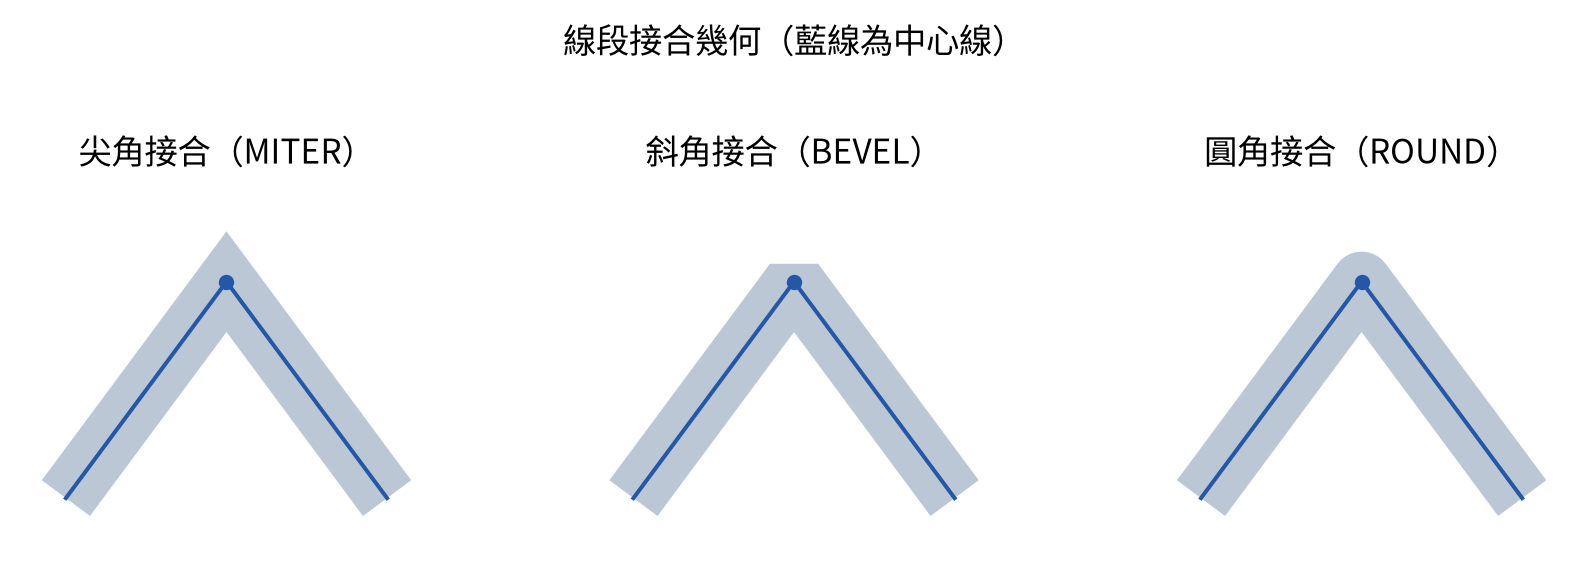
\includegraphics[width=\linewidth]{docs/figures/ch04_stroke-join.png}
        \caption{MITER、BEVEL 與 ROUND join}
        \label{fig:stroke-joins}
    \end{subfigure}\hfill
    \begin{subfigure}[t]{.43\textwidth}
        \centering
        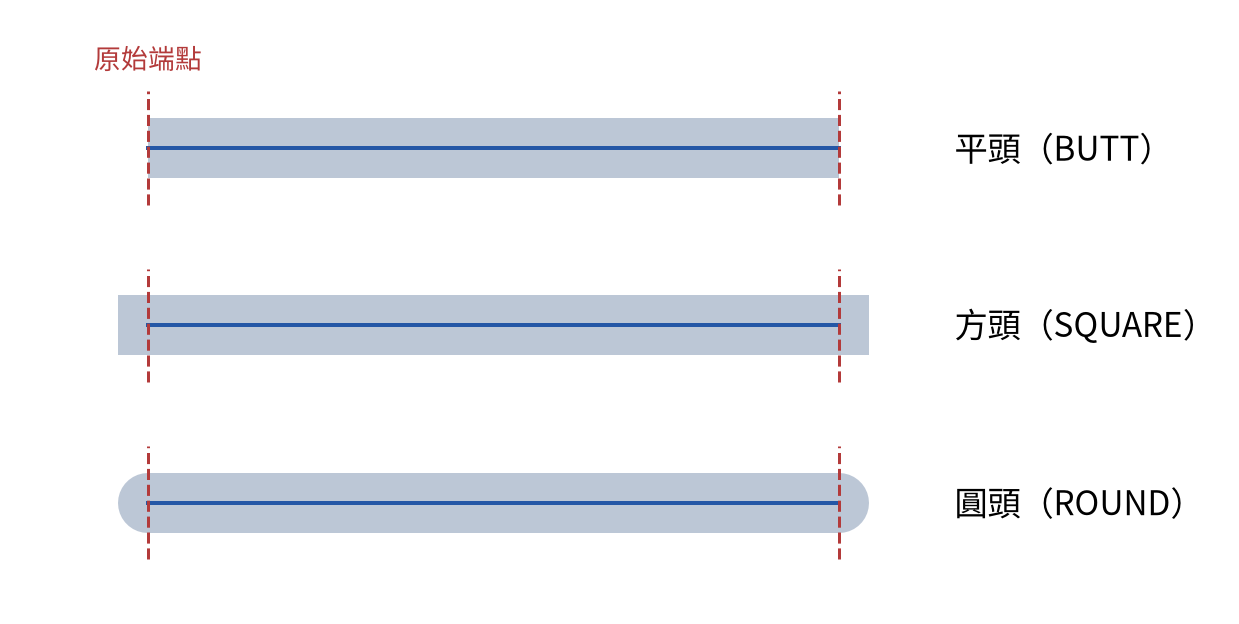
\includegraphics[width=\linewidth]{docs/figures/ch04_stroke-cap.png}
        \caption{BUTT、SQUARE 與 ROUND cap}
        \label{fig:stroke-caps}
    \end{subfigure}
    \caption{自行產生的筆畫接合與端點；細線或虛線表示中心線}
\end{figure}

當兩段線形成很尖的角度時，外側 offset line 的交點可能離 $B$ 很遠。程式將這段距離記為 miter length $m$，並與 $hL$ 比較，其中 $L$ 是 miter limit，目前預設為 4：

\[
    \text{使用 MITER 的條件：}\qquad m \leq hL.
\]

若 $m>hL$，即使使用者選擇 MITER，程式仍改用 BEVEL，避免出現過長的尖刺。圖~\ref{fig:miter-limit} 顯示這項判斷。

\begin{figure}[tbp]
    \centering
    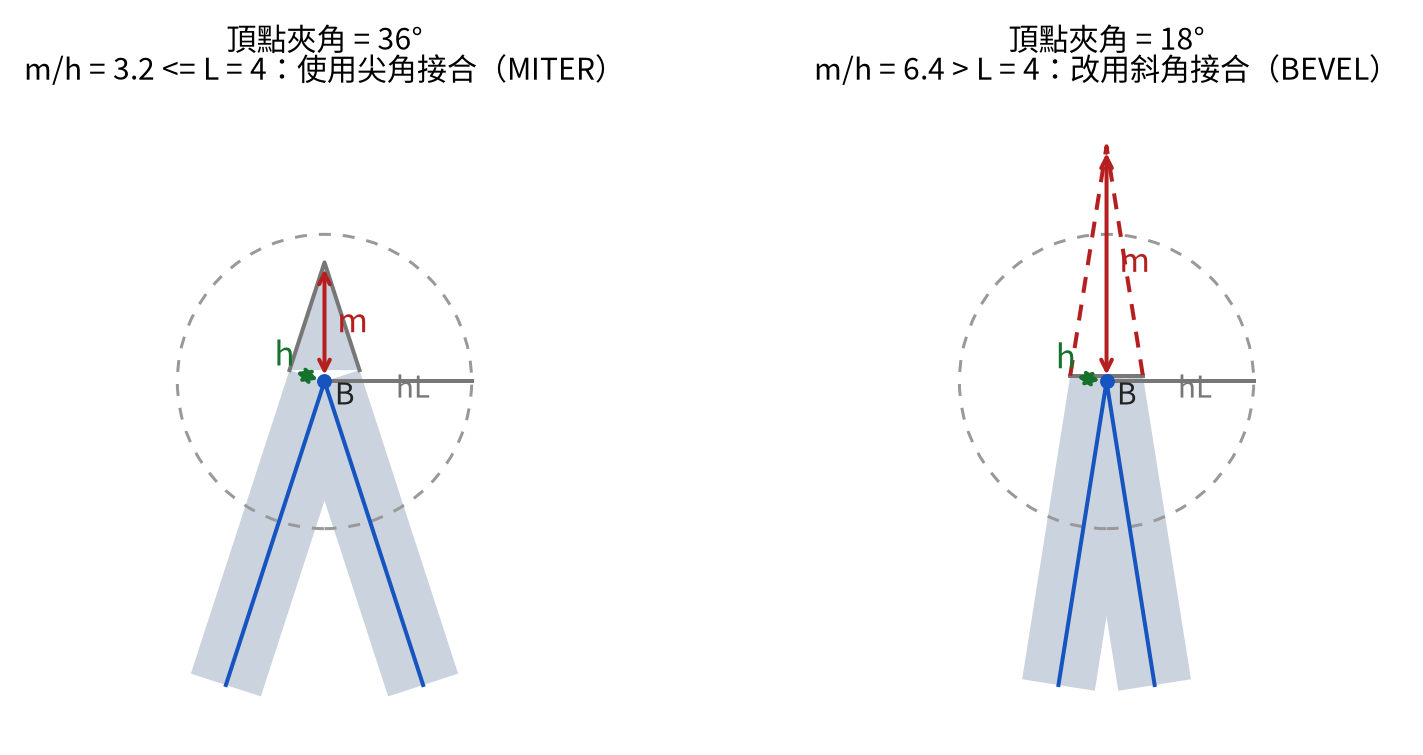
\includegraphics[width=.92\textwidth]{docs/figures/ch04_miter-limit.png}
    \caption{Miter limit 的實際轉角案例；灰底表示筆畫寬度，藍線為中心線}
    \label{fig:miter-limit}
\end{figure}

程式也處理平行、近 180 度折返與過遠 inner intersection。若 offset line 無法穩定求交，Join 退回 BEVEL 或 ROUND；inner intersection 超過附近 segment 長度與半寬推導出的限制時，改用原 vertex，避免短筆畫出現異常 triangle。

\subsection{Fill Rendering}

OUTLINE 與 FILLED 模式直接使用 OpenGL primitive 和 \lstinline|glPolygonMode()|。ADVANCED 模式則把填色與描邊分開：封閉圖形先填入 Fill color，再畫出自行計算的 Stroke geometry。若 Fill color 完全透明或頂點少於三個，就跳過填色。目前填色仍使用 \lstinline|GL_POLYGON|，因此凹多邊形可能無法得到正確結果，這部分尚未加入 triangulation。

\subsection{座標系統}

程式以 \lstinline|glOrtho(0, width, height, 0, -1, 1)| 將 UI、滑鼠與 Scene 統一為左上角原點。Canvas 再沿 parent chain 將視窗座標轉成局部座標，因此工具收到的位置、Scene 儲存的頂點與狀態列顯示一致；只有 framebuffer pixel I/O 仍採 OpenGL 的左下角順序，細節見附錄~\ref{app:framebuffer-details}。

\subsection{Grid}

Grid 只提供位置參考，不會加入 Scene 或改變物件頂點。Lines 與 Dots 模式都以 25 px 為間距，None 則不繪製；CanvasRenderer 會先畫 Grid，再畫 Scene、draft 與選取框，使格線保持在背景。
